\subsection{Intuition}
\label{sec:intuition}

To see a possible advantage of utilizing more fine-grained (non-root)
concepts and combining the results versus directly learning the
coarse-grained (root) concept, consider the simple example of
Figure~\ref{fig:unionex}.  In the figure, the coarse-grained concept
to be learned is circles (positives) versus diamonds (negatives).
If one limits the set of possible classifiers $\cal C$ to the set
of single axis-parallel boxes, then any hypothesis that has high recall
will have low precision.  However, if it is the case that the set
of positive instances can be decomposed into fine-grained classes
such as the four separate types of circles in Figure~\ref{fig:unionex},
then we can map the problem of classifying circles versus diamonds
into the four problems of classifying green solid circles versus
everything else, classifying blue open circles versus everything
else, and so on.  We could thus train four fine-grained classifiers,
one per circle type.  With these inferred fine-grained classifiers
in hand, one can make a prediction on a new instance by predicting
its membership in each of the four fine-grained classes and then
returning a prediction of circle if any of the fine-grained classifiers
predicts `yes'.  

Put another way, our approach takes advantage of a natural decomposition of the
general class into finer, possibly simpler sub-classes.  If the sub-classes
are in fact simpler to learn, then we can more easily learn the general class
by first learning the sub-classes and combining the sub-class predictions via, e.g., the 
union operator.  Since the union of hypotheses is a larger, more general
hypothesis space that includes the space of original hypotheses, this lends us
a potentially strong advantage in terms of representational ability.

\begin{figure}[ht]
\vskip 0.2in
\begin{center}
\centerline{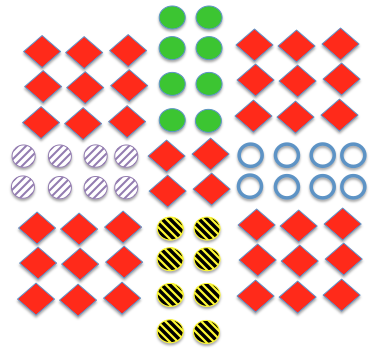
\includegraphics[width=\columnwidth]{fig/union.png}}
\caption{ An example of the potential usefulness of learning multiple
fine-grained concepts to support
the learning of a single coarse-grained one.  The negative instances are diamonds and the
positive ones are circles.  Each size-8 cluster of circles represents a separate fine-grained
concept within the general class of circles.}
\label{fig:unionex}
\end{center}
\vskip -0.2in
\end{figure} 

Of course, real learning problems may not be as simple to decompose
as that in Figure~\ref{fig:unionex}, but our experiments reveal
clear empirical advantages in precision for the same value of recall.
However, such fine-grained labels might be more 
expensive to obtain.  For example, when asked to label a phrase
of text, a human labeler can probably distinguish the name of an
attraction from that of a lake more easily than distinguish the
name of a park from that of a zoo.  Hence, we study how one can
combine the use of labels at different labels to effectively learn
the level-1 concept.

\subsection{Learning-Theoretic Advantages}
\label{sec:learningtheory}

More formally, one can express advantages of hierarchical labeling
over non-hierarchical labeling in terms of computational complexity,
sample complexity, and label complexity.   Below we summarize some
of these advantages in both the {\em probably approximately correct
(PAC)} and {\em exact} models of learning~{v-tl-84}.  In the PAC
model, a learner is given positive parameters $\epsilon < 1/2$ and
$\delta < 1/2$ and access to a set of labeled training instances
drawn iid according to an arbitrary distribution $\cal D$.  The
learner  is then expected, in polynomial time, with probability at
least $1-\delta$, to output a hypothesis  that has error at most
$\epsilon$ on new instances drawn according to $\cal D$.  In the
exact learning model, the learner gets access to two oracles: a
{\em membership query} (MQ) oracle and an {\em equivalence query}
(EQ) oracle.  An efficient learner will learn the exact identity
of the target concept in time and number of queries that are
polynomial in the problem size.  When the learner poses an EQ, it
passes to the oracle a hypothesis $h$ that it thinks is exactly
equivalent to the target concept, i.e., that will label all instances
exactly correctly.  The oracle either responds that the hypothesis
is exactly correct or gives to the learner a counterexample, which
is an instance on which $h$ is wrong.  An MQ oracle receives from
the learner an instance $x$ and provides $x$'s label.  It is similar
to an active learning model, except that in the MQ model, the
instances can be arbitrary while in AL, the instances must come
from a pre-specified set.

In the context  of computational complexity, we consider the case
(in both the PAC and exact learning models) of {\em proper}
learning\footnote{Note that the negative results described below for both
exact and PAC learning are only for proper learning.  One can get
positive results for these cases by allowing a logarithmic increase
in the number of boxes used, by applying the set cover approximation
algorithm.}.
Proper learning is when the training instances are labeled by a
concept from $\cal C$ and the hypothesis inferred by the learner
is required to also be from $\cal C$.
We will consider the passive (where all instances are labeled)
proper learning of axis-parallel boxes,
in a bounded, discretized, $d$-dimensional instance space $\{0,\ldots,t-1\}^d$ for
exact learning and the real space $\mathbb{R}^d$ for PAC learning.

For exact learning, we have from Bshouty and Burroughs~\cite{bb-plapc-03}
that one cannot exactly properly learn $k$-unions of boxes when (constant) $d>2$ unless 
P $=$ NP.  I.e., while one can learn $k$-unions with $O(d \log k)$-unions, one cannot 
efficiently learn $k$-unions with $k$-unions  if P $\ne$ NP.  In contrast, if we
use fine-grained labels for $k$ distinct fine-grained hypotheses (each using one 
box), one can exactly learn each box individually with one EQ (to get a positive
instance) and $O(d \log t)$ MQs (for binary search to find the box's $2d$ boundaries), for a
total of $O(k)$ EQs and $O(kd \log t)$ MQs and time polynomial in the number of queries.
Note that the positive result for fine-grained works for non-constant $d$, while the
hardness result for direct proper learning holds for even constant $d$.

For PAC learning boxes in $\mathbb{R}^d$, we use a result from Blumer et al.~\cite{behw-lvd-89}
that a concept class $\cal C$ is properly PAC learnable  if and only if there exists an 
algorithm to find a hypothesis from $\cal C$ consistent with a labeled training sample 
(this is called the {\em consistent hypothesis problem}).
In other words, if RP $\ne$ NP, then when the consistency problem for $\cal C$ is NP-hard,
$\cal C$ is not properly PAC learnable.
Since it is NP-hard to find a smallest
set of rectangles to cover a set of points in $\mathbb{R}^d$ even
for $d=2$~\cite{behw-lvd-89,m-sncscp-xx},
this implies  that one cannot properly PAC learn $k$-unions of boxes.
In contrast, using fine-grained labels, one can simply learn $k$ single boxes, one
at a time, which can easily be done in time $O(kdn)$.

In the context of sample complexity, we look at passive PAC learning of unions of $k$
axis-parallel boxes in $\mathbb{R}^d$.  The
classic approach~\cite{behw-lvd-89} to PAC learning a function class $\cal C$ is to
draw a labeled sample $\cal X$ of size  at least
\begin{equation}
m(\epsilon,\delta) = \max \left( {2 \over \epsilon} \log {2 \over \delta}, {8D \over \epsilon} \log {13
\over \epsilon}  \right)
\enspace ,
\label{eqn:behw}
\end{equation}
where $\epsilon$ and $\delta$ are the PAC parameters and $D$ is
the VC-dimension (VCD) of $\cal C$,
and to then find some function $c \in {\cal C}$ consistent with
$\cal X$.  

The VC-dimension of the class of single $d$-dimensional axis-aligned boxes is $2d$.  Based on
Blumer et al.~\cite{behw-lvd-89}, then, the VCD of the $k$-union of
$d$-dimensional axis-aligned boxes is
$\Theta(d  k \log k)$.  Thus, to directly PAC-learn $k$-unions of $d$-dimensional boxes,
it suffices to find a hypothesis consistent with 
\[
m_{coarse}(\epsilon,\delta) = \Theta \left( {1 \over \epsilon} \log {1 \over \delta}
+ {d k \log k \over \epsilon} \log {1 \over \epsilon}  \right)
\enspace 
\]
labeled examples\footnote{Note that we are not considering the time complexity of finding such
a consistent hypothesis, only the number of training instances.}.
In contrast, learning the class of individual $d$-dimensional boxes reduces
the VCD from $\Theta(d  k \log k)$ to $\Theta(d)$.  However, since the learning
process is repeated $k$ times, one needs to learn each individual box with a smaller value of
$\epsilon$ and a smaller value of $\delta$,
to allow for the union bound to be applied across all $k$
fine-grained hypotheses.  This yields a sample complexity of 
\[
m_{fine}(\epsilon/k,\delta/k) = \Theta \left( {k \over \epsilon} \log {k \over \delta}
+ {d k  \over \epsilon} \log {k \over \epsilon}  \right)
\enspace 
,
\]
which grows more slowly than $m_{coarse}$.
%  since  $m_{coarse}-m_{fine}$ is positive.

We now consider label complexity, in which one wants to minimize the 
number of labels purchased by an active learning algorithm.
We will work in a model where we are given the training data $\cal X$, but initially
the labels are missing.  This is exactly active learning, and the question
we ask is: how many label purchases
are necessary/required to find a consistent hypothesis, assuming one exists? 

For this example, we will let $\cal C$ be the set  of unions of at
most $k$ disjoint intervals on $\mathbb{R}$. When a coarse-grained label
of an instance $x \in {\cal X}$ is purchased, it comes back as
`$+$' if $x$ lies in one of the $k$ target intervals and `$-$' otherwise.
When a fine-grained label of $x$ is purchased, the label is an indicator
of which of the $k$ target intervals it lies in ($I_1,\ldots,I_k$) or `$-$' if
it does not lie in any of the target intervals.  We assume that there is
at least one point from $\cal X$ in each interval $I_j$ and that there is
at least  one point from $\cal X$ between each adjacent pair of intervals
(otherwise, those empty intervals/gaps between intervals are irrelevant in
the PAC sense).

We now analyze both the coarse-grained and fine-grained active learning
models in this context. Assume that, for each target interval, there is
one instance of  $\cal X$ that is pre-labeled (for free).  I.e., in the 
coarse-grained case, there are $k$ instances labeled `$+$' (one in each target
interval) and in the fine-grained case there is one instance labeled $I_1$,
one labeled $I_2$, etc. In this case, clearly an algorithm in the coarse-grained
model can use the free labels to infer the identity of one point per interval.

The goal of an algorithm in either labeling model is to find the
left and right boundaries of each of the $k$ target intervals, which
is tantamount to identifying the leftmost and rightmost negatively
labeled points between each consecutive pair of intervals.  Consider
two consecutive intervals $I_j$ and $I_\ell$ that, when taken
together and their intervening gap, contain the largest number of
points from $\cal X$ of all consecutive pairs of intervals.  Since
it is the largest number of points, this count has to be $\Omega(m/k)$
but could be $O(m)$ in the worst case.  Now consider an algorithm
that operates only with coarse-grained labels.  In searching for
the set of negative points from $\cal X$ lying between $I_j$ and
$I_\ell$, it will purchase the label of some point $>x_j$ and
$<x_\ell$, where $x_j$ and $x_\ell$ are the pre-labeled points from
$\cal X$ from $I_j$ and $I_\ell$, respectively (any other queries
are superfluous).  In the worst case, an adversary will simply
answer `$+$' to any such query, until only one remains to be labeled
`$-$'.  This will require $\Omega(m)$ queries in the worst case.

On the other hand, an algorithm in the fine-grained labeling scheme
can perform a binary search between $x_j$ and $x_\ell$  (now labeled
$I_j$ and $I_\ell$) until a negatively labeled instance $x_-$ is found.  When
that is done, simply perform two binary searches: one between $x_-$ and
the right-most point in $I_j$ and one between $x_-$ and
the left-most point in $I_\ell$. This takes at most $O(\log m)$ queries
per pair of intervals, for a total of $O(k \log m)$ queries.


Since the VC dimension $D$ of the union of $k$ intervals is $2k$, we will need
$\cal X$ of size 
\[
m \ge \max \left( {2 \over \epsilon} \log {2 \over \delta}, {16 k \over \epsilon} \log {13
\over \epsilon}  \right)
\enspace .
\]
Ignoring the first term of the max, this means that our worst-case lower bound 
of purchases for a coarse-grained learner is $\Omega ((k / \epsilon ) (\log 1/\epsilon))$,
while our worst-case upper bound of purchases for a fine-grained learner is
$O(k \log (k/\epsilon) + k \log \log (1/\epsilon))$. Both are linear in $k$ but the
coarse-grained learner's bound is worse by a factor  exponential in $1/\epsilon$.

